\documentclass[../main.tex]{subfiles}

\begin{document}
	\section{Rappresentazione dei sistemi lineari}
	Un sistema SISO può essere rappresentato in due modi:
	\begin{enumerate}
		\item con un'equazione lineare a coefficienti costanti (vedi \ref{eq_diff_lin}).
		\item con la funzione di trasferimento $ T(s) = \frac{\bar{B}(s)P(s)}{\bar{A}(s)P(s)} $.
	\end{enumerate}
	Dall'equazione differenziale si ottiene univocamente una funzione di trasferimento.\\
	Il passaggio inverso non \'{e} univoco perch\'{e} possiamo introdurre un polinomio $ P(s) $ arbitrario.\\
	%
	\paragraph{Esempio}
	\[ T(s) = \frac{1}{s+1} \qquad \begin{array}{l} \bar{B}(s) = 1\\ \bar{A}(s) = s+1 \end{array} \]
	Ma se considero i polinomi $ A(s) $ e $ B(s) $ prima della semplificazione dei fattori comuni:
	\[ \begin{array}{l} B(s) = 1 \cdot P(s)\\ A(s) = (s+1)P(s) \end{array} \qquad \forall P(s) \]
	\begin{itemize}
		\item $ P(s) = s $
		\[ \begin{array}{l} B(s) = s\\ A(s) = s^2+s \end{array} \qquad \Rightarrow \qquad \ddot{y}(t) + \dot y(t) = \dot u(t)\]
		\item $ P(s) = s-1 $
		\[ \begin{array}{l} B(s) = s-1\\ A(s) = s^2-1 \end{array} \qquad \Rightarrow \qquad \ddot{y}(t) - y(t) = \dot{u}(t) - u(t)\]
		\item $ P(s) = 1 $ scelta \textit{standard}
		\[ \begin{array}{l} B(s) = 1\\ A(s) = s+1 \end{array} \qquad \Rightarrow \qquad \dot{y}(t) + y(t) = u(t)\]
		\item $ P(s) = 3 $ basta dividere per la costante e si ottiene l'equazione differenziale cercata
		\[ \begin{array}{l} B(s) = 3\\ A(s) = 3s+3 \end{array} \quad \Rightarrow \quad 3\dot{y}(t) + 3y(t) = 3u(t) \quad \Rightarrow \quad \dot{y}(t) + y(t) = u(t)\]
	\end{itemize}
	Quindi la rappresentazione di un sistema con l'equazione differenziale \'{e} pi\'u completa perch\'e univoca, mentre l'altra introduce arbitrariet\'a. Il passaggio da $ T(s) $ a equazione differenziale \'e univoco se e solo se \'e anche specificato l'ordine $ n = \bar n $ ($ \bar n = \pDeg{\bar A(s)} $) del sistema.\\
	\smallskip\\
	\'E prassi comune descrivere sistemi dinamici attraverso la funzione di trasferimento $ T(s) $. (\'e lecito se non ci sono parti nascoste). Se non \'e scontato che non esistano parti nascoste, allora $ T(s) $ d\'a informazioni solo riguardo la risposta forzata, ma nulla della risposta libera. \'E pericoloso se la parte nascosta non \'e stabile.\\
	%
	\paragraph{Esempio} supponiamo di avere il seguente sistema di cui ci danno la funzione di trasferimento $ T(s) = \frac{1}{s+1} $, mentre il sistema 2 \'e nascosto:\\
	\begin{figure}[h!]
		\begin{subfigure}{0.5\textwidth}
			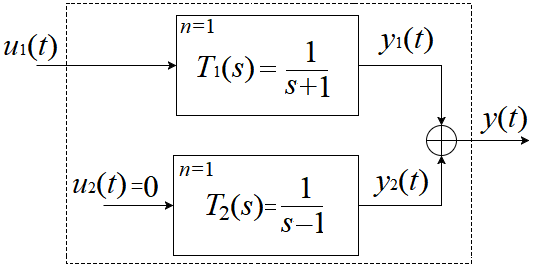
\includegraphics[width=8cm, height=4cm]{sistema_nascosto}
		\end{subfigure}
		\begin{subfigure}{0.5\textwidth}
			\begin{align*}
				&Y(s) = Y_1(s) + Y_2(s) =\\
				&= \underbrace{T_1(s)U_1(s) + T_2(s)U_2(s)}_{Y_f(s)} + \underbrace{\frac{I_1(s)}{s+1} + \frac{I_2(s)}{s-1}}_{Y_l(s)}
			\end{align*}
		\end{subfigure}
	\end{figure}
	\newpage\noindent
	Poich\'e $ U_2(s) = 0 \quad \Rightarrow \quad Y(s) = Y_f(s) = T_1(s)U_1(s)$:
	\begin{itemize}
		\item La risposta forzata \'e stabile per qualunque ingresso, perch\'e l'unico polo \'e a $ \Re < 0 $.
		\item La risposta libera ha un polo $ s = 1 $ $ (\Re > 0) $, quindi \'e instabile se le condizioni iniziali non sono nulle $ I_2(s) \neq 0 $.
	\end{itemize}
	In conclusione la funzione di trasferimento fornita non ci d\'a alcuna informazione sulla parte nascosta.\\ 
\end{document}